\documentclass[12pt]{article}

% language stuff
% \usepackage{ngerman}           % deutsche Überschriften etc.
\usepackage{german}
\usepackage[utf8]{inputenc} % direkte Einbgabe von Umlauten

% Layout-Einstellungen
\usepackage{parskip}          % Abstand statt Einrückung
\frenchspacing                % no extra space after periods
\usepackage{parskip}          % paragraph gaps instead of indentation
\usepackage{times}            % default font Times
\tolerance=9000               % avoid words across right border

% miscellaneous
\usepackage{graphicx}         % graphics
\usepackage{hhline}           % double lines in tables
\usepackage{amsfonts}         % real numbers etc.
\usepackage[rightcaption]{sidecap} % figure captions on the right (optional)
\usepackage{hyperref}         % for URLs
\usepackage{listings}         % for code samples

% Hier bei Bedarf die Seitenränder einstellen
\usepackage{geometry}
%\geometry{a4paper}
\geometry{a4paper,left=25mm,right=25mm, top=3.0cm, bottom=3.0cm} 

% Paragraph Änderung
\usepackage{color,soul}
\usepackage{titlesec}

\setcounter{secnumdepth}{4}

\titleformat{\paragraph}
{\normalfont\normalsize\bfseries}{\theparagraph}{1em}{}
\titlespacing*{\paragraph}
{0pt}{3.25ex plus 1ex minus .2ex}{1.5ex plus .2ex}
%
%%%%%%%%%%%%%%%%%%%%%%%%%%%%%%%%%%%%%%%%%%%%%%%%%%%%%%%%%%%%%%
\title{\vspace*{-10mm}Analyse eines C++-Programms\\ zur Simulation von Mehrphasenströmungen}
\author{
	% Autor und Email-Adresse ersetzen:
	Pascal Bähr
	}

\date{14. April 2016}

%%%%%%%%%%%%%%%%%%%%%%%%%%%%%%%%%%%%%%%%%%%%%%%%%%%%%%%%%%%%%%
\begin{document}

\maketitle

%-------------------------------------------------------------
\begin{abstract}
%-------------------------------------------------------------
Zum besseren Verständnis des Programms soll dieses Dokument dienen. Die Funktionalitäten und die verwendeten Datenstrukturen der einzelnen Klassen werden übersichtlich und verständlich erläutert, so dass eine spätere Umstrukturierung des Programms einfacher wird. Es wird zunächst nur die Implementierung für eine Dimension betrachtet. Referenzen zu Gleichungen beziehen sich auf die zur Verfügung stehende Zusammenfassung des Themas.
\end{abstract}



%=============================================================
\section{Ablauf}
Der grobe Ablauf des Programms.
\begin{enumerate}
	\item Auswahl der Methode zur Flußberechnung $|$ main
	\item Auswahl Splitting/Unsplitting $|$ numerische\_methode
	\item Solange keine Abbruchbedingung erfüllt worde (maximale Schritte,maximale Zeit)
	\begin{enumerate}
		\item Setzen der Randbedingungen (Boundary Conditions) $|$ numerische\_methode $\rightarrow$ raster
		\item Zeitschritt über höchsten Eigenwert berechnen $|$ numerische\_methode . cflcon()
		\item Update Schritt
		\begin{enumerate}
			\item Fluss über gewählte Methode berechnen (U \& F $\rightarrow F^{LF}$)
			\item Updateschritt berechnen mit dem berechneten Fluss
			\item Zellwerte aktualisieren
		\end{enumerate}	
	\end{enumerate}	
	\item Ergebnisse exportieren
\end{enumerate}	

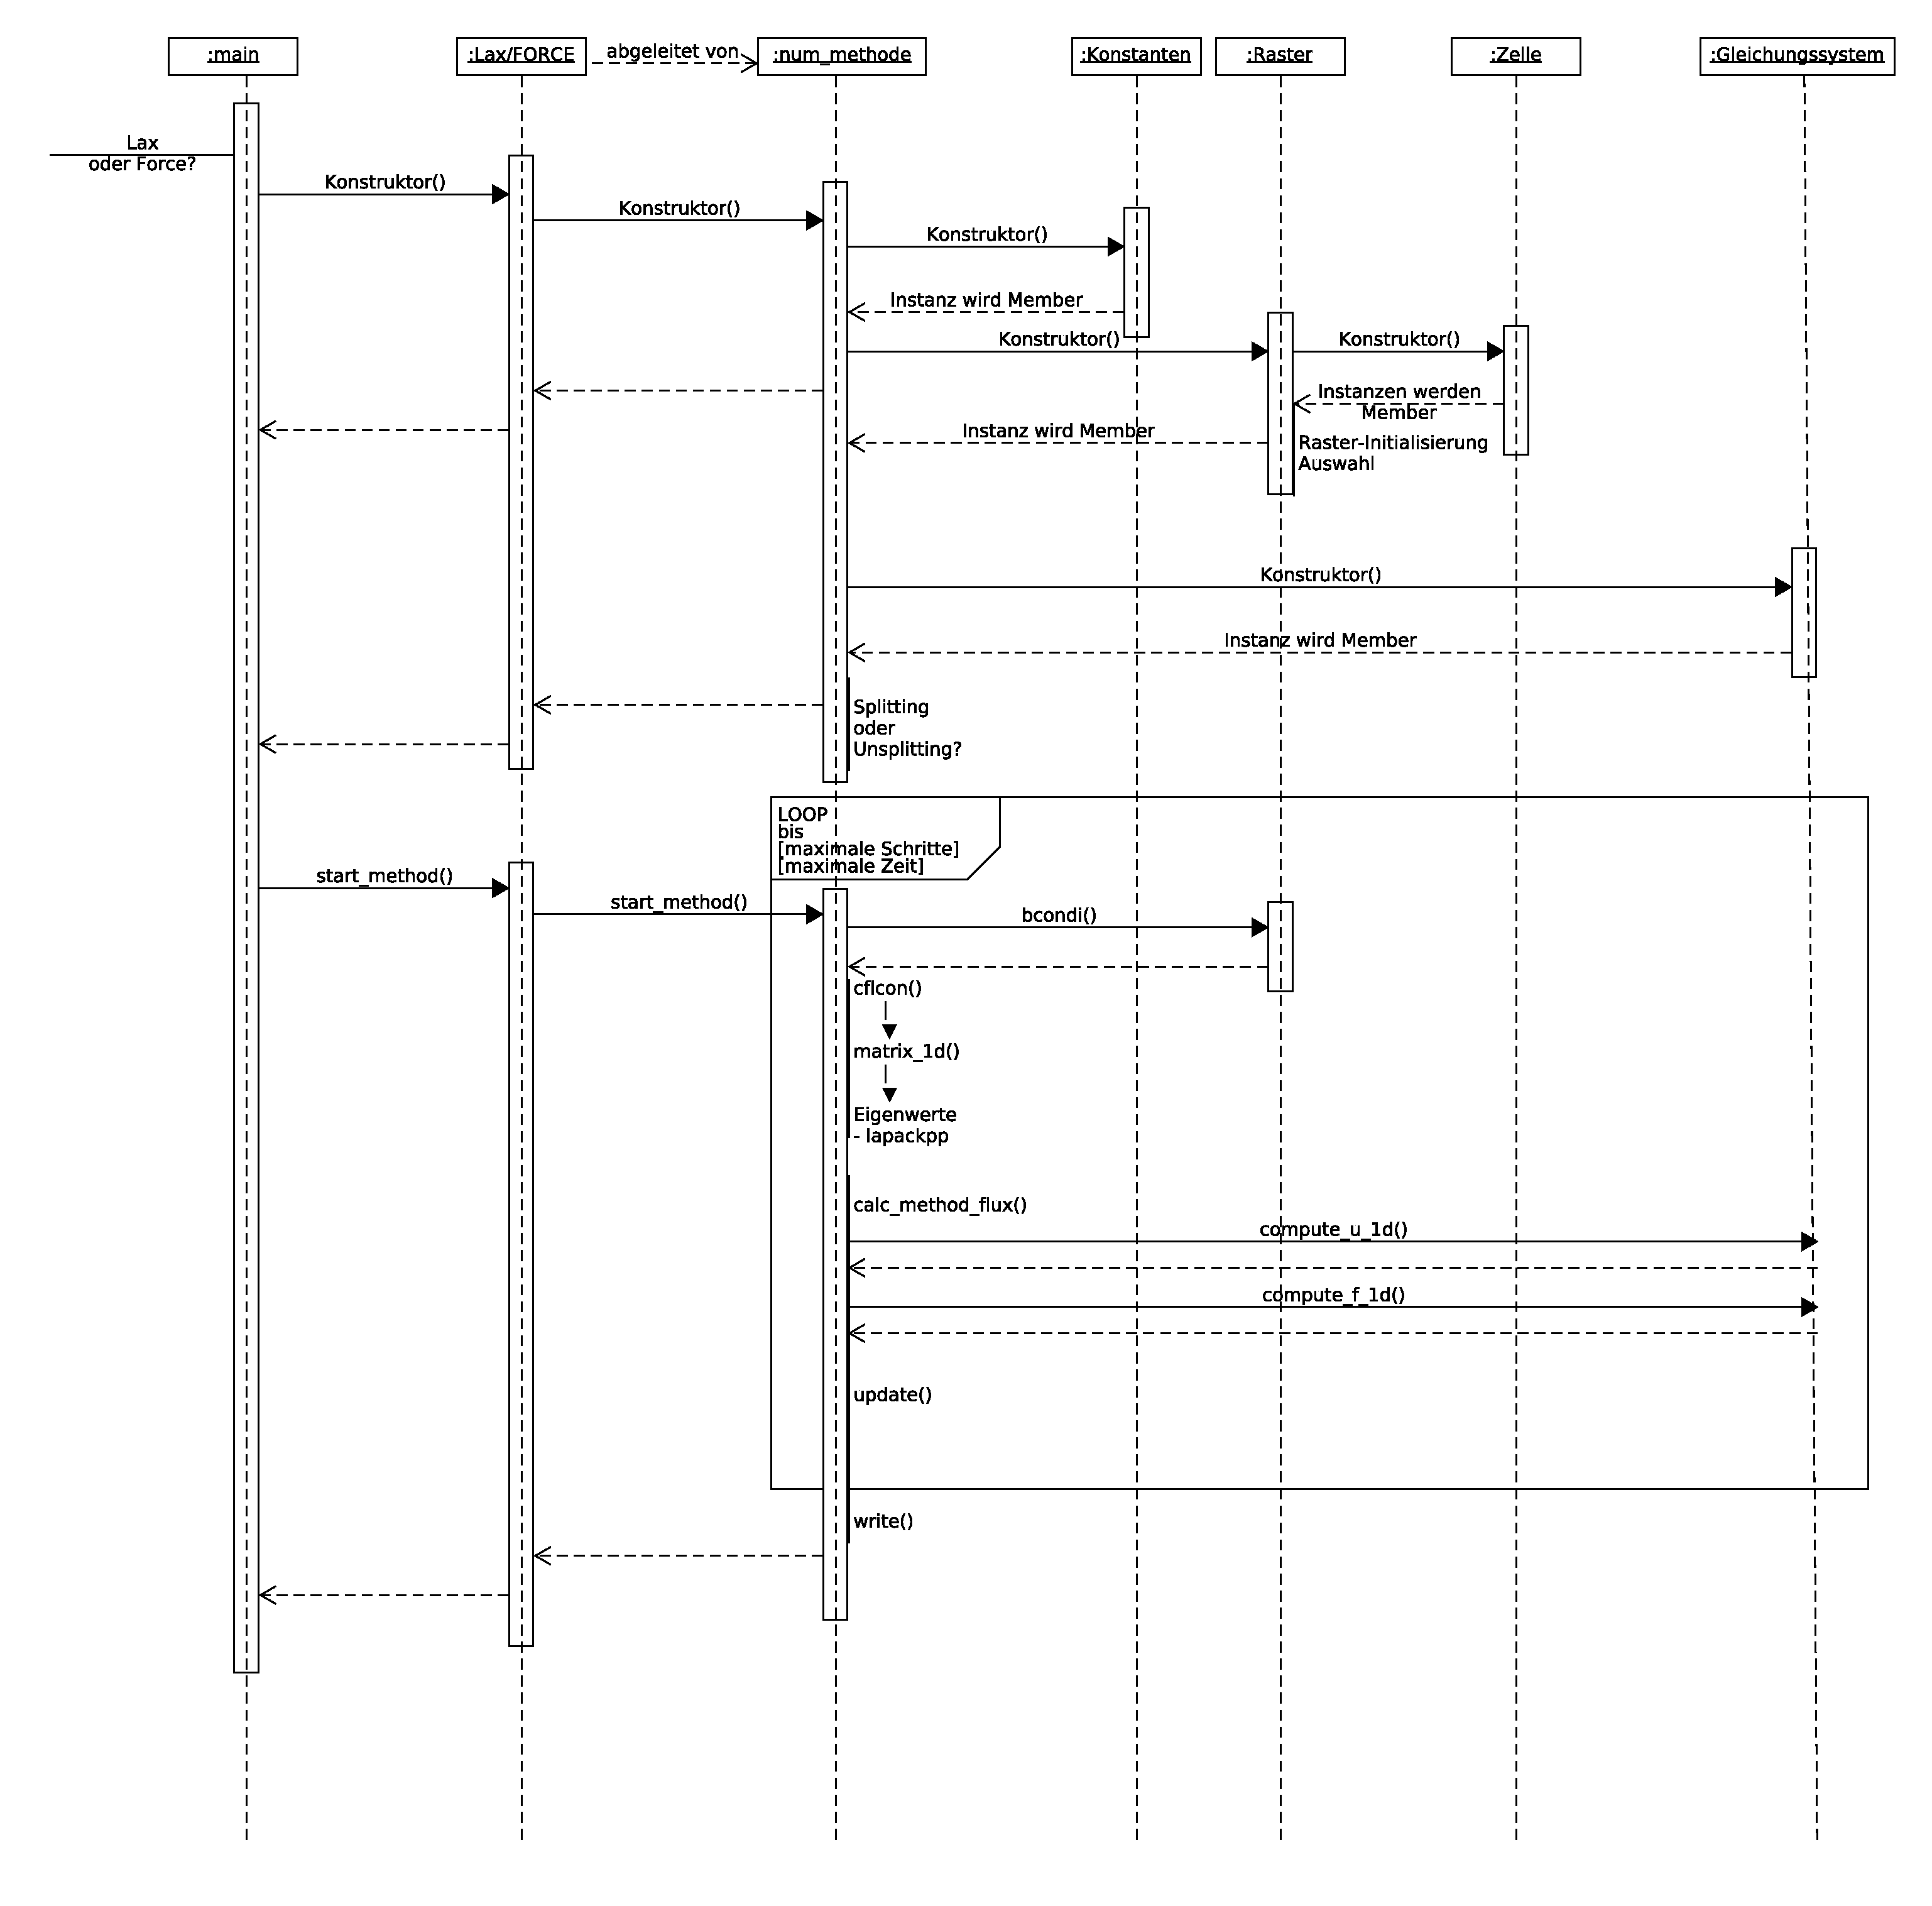
\includegraphics[scale=0.3]{multiflow_sequenz}

%-------------------------------------------------------------
% default a), b), c) numbering
\renewcommand{\labelenumi}{\alph{enumi})} 

\section{Dateien}
%-------------------------------------------------------------
\subsection{main.cpp}
Dient bisher nur zur Auswahl der Flußberechnungsmethode. \\
Zur Auswahl stehen:
\begin{enumerate}
	\item Lax-Friedrich Methode
	\item FORCE Methode
\end{enumerate}

\subsection{LaxFriedrichMethode.*}
Abgeleitet von der Klasse {\em numerische\_methode}\\
Verwendet Konstruktor der Basisklasse \\
Implementiert die abstrakte Methode {\em calc\_method\_flux()} \\

\subsubsection{calc\_method\_flux()} \label{sssec:laxcalc}
Parameter {\em int dir} sollte implementiert werden, damit (ab 2 Dimensionen) nicht immer beide Flüsse F und G (pro Richtung) berechnet werden müssen
\paragraph{Variablen}
Zunächst Initialisierung einiger Variablen:
\begin{enumerate}
	\item width \& height: Mit Werten der Größe des Rasters
	\item neqs: Anzahl der Gleichungen aus Gleichungssystem-Klasse, bei 1 Dimension -"> 3
	\item *uall/*fall/*gall: 
	\\Allokierung eines Arrays für zusammenhängenden Speicher
	\item ***cs/***f/***g: 
	\\3D-Arrays der Größe 'neqs X width X height'
	\\Mit zusammenhängen Speicher in allen Dimensionen über Array uall... + Speicherarithmetik
	\item 4-facher Vektor fi: 
	\\ Return Vektor für $F_{i}$ bei der Flussberechnung
	\\ in etwa wie: a[i][j][k][l]
	\\ i = neqs
	\\ j = Raster Width
	\\ k = Raster Heigth
	\\ l = Dimension, also 1 oder 2, später auch 3
	\\ alle Werte initialisiert mit 0.0
\end{enumerate}

\renewcommand{\labelenumi}{\theenumi.} 
\paragraph{Algorithmus}
Eigentliche Fluss-Berechnung:\\
\begin{enumerate}
	\item U Berechnen durch Gleichungssystem-Klasse
	\item F Berechnen durch Gleichungssystem-Klasse
	\item L-F Fluss $F^{LF}$ berechnen über Gleichung 5.50\\
	\begin{equation}
	F^{LF}_i = \frac{1}{2}\left(F_i^n+F_{i+1}^n \right) + \frac{\Delta x}{2
		\Delta t}\left(U_i^n - U_{i+1}^n \right)\label{eq:fluss_LF}
	\end{equation}
	$F^{LF}_i$ ist eine Iteration über (in Array-Schreibweise): fi[k][i][0][0]\\
	k := 0 bis neqs\\
	i := 0 bis CELLS[0]+ordnung+1\\
	\textcolor{red}{Besser raster.getwidth() - ordnung\\
	Die Raster Höhe und die Dimension bei der 1-D Berechnung sind quasi überflüssig.}
	\item Rückgabe des Vektorkonstruktes
\end{enumerate}

\subsection{FORCE.*}
Abgeleitet von der Klasse {\em numerische\_methode}\\
Verwendet Konstruktor der Basisklasse \\
Implementiert die abstrakte Methode {\em calc\_method\_flux()} \\

\subsubsection{calc\_method\_flux()} \label{sssec:forcecalc}
Parameter {\em int dir} sollte implementiert werden, damit (ab 2 Dimensionen) nicht immer beide Flüsse F und G (pro Richtung) berechnet werden müssen
\paragraph{Variablen}
Zunächst Initialisierung einiger Variablen:
\begin{enumerate}
	\item width \& height: Mit Werten der Größe des Rasters
	\item neqs: Anzahl der Gleichungen aus Gleichungssystem-Klasse, bei 1 Dimension $\rightarrow$ 3\\
	\textcolor{red}{Anzahl der Gleichungen dürfte pro Dimension nicht fix sein!}
	\item *uall/*fall/*gall/*f\_laxall/*f\_rieall/*g\_laxall/*g\_rieall: 
	\\Allokierung eines Arrays für zusammenhängenden Speicher
	\item ***cs/***f/***g/***f\_lax/***f\_rie/***g\_lax/***g\_rie: 
	\\3D-Arrays der Größe 'neqs X width X height'
	\\Mit zusammenhängen Speicher in allen Dimensionen über uall... + Speicherarithmetik
	\item 4-facher Vektor fi: 
	\\ Return Vektor für $F_{FORCE}$ bei der Flussberechnung
	\\ wie a[i][j][k][l]
	\\ i = neqs
	\\ j = Raster Width
	\\ k = Raster Heigth
	\\ l = Dimension, also 1 oder 2
	\\ alle Werte initialisiert mit 0.0
\end{enumerate}

\renewcommand{\labelenumi}{\theenumi.} 
\paragraph{Algorithmus}
Eigentliche Fluss-Berechnung:\\
\begin{enumerate}
	\item U Berechnen durch Gleichungssystemklasse
	\item F Berechnen durch Gleichungssystemklasse
	\item Lax-Friedrichs Fluss $F^{LF}$ berechnen über Gleichung 5.50\\
	\begin{equation}
	F^{LF}_i = \frac{1}{2}\left(F_i^n+F_{i+1}^n \right) + \frac{\Delta x}{2
		\Delta t}\left(U_i^n - U_{i+1}^n \right)\label{eq:fluss_LF}
	\end{equation}
	$F^{LF}_i$ ist eine Iteration über (in Array-Schreibweise): fi[k][i][0][0]\\
	k := 0 bis neqs\\
	i := 0 bis CELLS[0]+ordnung+1\\
	\textcolor{red}{Besser -$>$ raster.getwidth() - ordnung\\
	Fluss wird ein zweites mal über eine Vektor Länge (aus Gleichungssystem) berechnet, wahrscheinlich ein Artefakt!}
	\item Richtmeyer Vektor $U^{RI}$ (als Raster aufgebaut) berechnen über Gleichung 5.53\\
	\begin{equation}
	U^{RI}_{i+1/2} = \frac{1}{2}\left[U_i^n + U_{i+1}^n\right] + \frac{\Delta t}{2
		\Delta x}\left(F_{i}^n - F_{i+1}^n \right) \label{eq:fluss_RI}
	\end{equation}
	Jeweils für jede Zelle: d (Dichte), ux (Geschwindigkeit in x-Richtung), uxr (Relative Geschwindigkeit in x-Richtung)\\
	Von Vektor U aus Gleichung 5.24:
	\[
	U =  \left[\begin{array}{c}\rho \\ \rho u \\ u_r\end{array}\right]
	\]
	bzw im Programm für die Werte der Zelle:
	\[
	U =  \left[\begin{array}{c}\rho \\ \frac{\rho u}{\rho} \\ u_r\end{array}\right]
	=  \left[\begin{array}{c}\rho \\ u \\ u_r\end{array}\right]
	=>  \left[\begin{array}{c}d \\ ux \\ uxr\end{array}\right]
	\]
	
	zusätzlich den Druck p (Druck) pro Zelle über Gleichung 5.15\\
	\begin{equation}
	P = K_g \rho^{\gamma},\label{eq:druck_rho}
	\end{equation}
	\item Richtmeyer Fluss $F^{RI}$ berechnen durch Gleichungssystemklasse. Veranschaulicht durch Gleichung 5.54\\
	\begin{equation}
	F^{RI}_{i+1/2} = F(U^{RI}_{i+1/2}) .
	\end{equation}\\
	\item FORCE Fluss $F^{FORCE}$ berechnen durch Mittelwert Berechnung zwischen den zwei Flüssen. Gleichung 5.55\\
	\begin{equation}
	F^{FORCE}_{i+1/2} = \frac{1}{2}\left[ F^{LF}_{i+1/2} +  F^{RI}_{i+1/2} \right]
	\end{equation}
	Gespeichert in f\_force Vektor
	\item Rückgabe des Vektorkonstruktes
\end{enumerate}

\renewcommand{\labelenumi}{\alph{enumi})} 
\subsection{numerische\_methode.cpp}
Basisklasse für die spezialisierten Flußberechnungsmethoden.\\
Beinhaltet die meiste Funktionalität des Programms.

\subsubsection{Konstruktor} \label{sssec:numkons}
\paragraph{Variablen}
Zunächst Initialisierung einiger Variablen durch auslesen aus Werten der Konstanten.\\
\textcolor{red}{Konstanten Klasse hat in der Implementierung keinen höheren Nutzen.}
\begin{enumerate}
	\item name: für Protokollierung mit write() \ref{sssec:write} zur Unterscheidung zwischen Lax-Friedrich und FORCE Methode
	\item ordnung: Ordnung des Verfahrens / \textcolor{red}{Wie viele zusätzliche Zellen an den Rändern miteinbezogen werden} /  bisher nur 1 implementiert
	\item dimension: Dimension in der gerechnet wird. Bisher 1D (x) und 2D (x,y)
	\item CELLS: Zeigt Anzahl der Zellen in entsprechender Dimension\\
	CELLS[0] für Zellen in X; CELLS[1] für Zellen in Y
	\item cref: Konstante in Equation of States; K$_2$
	\item done: Dichte der Phase 1; $\rho_1$
	\item ccl: Massenanteil in Simulation
	\textcolor{red}{\item mor: x-Wert rechte Grenze - oben rechts
	\item mol: x-Wert linke Grenze - oben links
	\item mur: y-Wert untere Grenze - unten rechts
	\item mul: y-Wert obere Grenze - unten links}
	\item timeou: Zeit Output - maximale Zeit als Abbruchbedingung
	\item steps: Zum Festhalten der gemachten Schritte zur Protokollierung
	\item maxnt: Gesetztes Maximum als Abbruchbedingung bei Fehler
	\item teilerend: für wieviel Schritte dt geteilt wird
	\item teiler: um wieviel dt zuerst geteilt wird\\
	klein Anfang für Stabilität
	\item variante: Variante der EOS \\andere varianten nicht getestet
	\item g: Gamma Konstante für EOS
	\item dx: Delta x ((rechter Rand-linker Rand)/Anzahl Zellen in x) / dy: Delta y
	\item dt: Delta t bei Berechnung des Time Steps mit CFL\\
	\textcolor{red}{zum Debuggen mit 0 initialisiert, sonst nicht vorher in Verwendung}
	\item rhol: Initialwert der Dichte der Phase 2, links
	\item alfll: Alpha-Berechnung (Volumenanteil) über 
	\[
	\alpha = 1 - \rho/\rho_1 + c\rho/\rho_1
	\]
	bzw im Programm
	\[
	alfll = 1.0 - rhol/done + ccl*rhol/done
	\]
	\textcolor{red}{Als Einzelschritt eigentlich unnötig, da nur für den nächsten Schritt benötigt wird}
	\item dll: Berechnung von Dichte $\rho_2$ über
	\[
	\rho_2 = (c\rho)/\alpha,
	\]
	bzw im Programm
	\[
	dll = ccl*rhol/alfll
	\]
	\textcolor{red}{Als Einzelschritt eigentlich unnötig, da nur für den nächsten Schritt benötigt wird}
	\item pll: Berechnung von Druck $P$ über
	\[
	P = K_2\rho_2^\gamma
	\]
	bzw im Programm
	\[
	pll = cref*dll^g
	\]
	\textcolor{red}{Als Einzelschritt eigentlich unnötig, da nur für den nächsten Schritt benötigt wird}
	\item ct: Berechnung der CT bzw $K_g$ Größe über (Umformung von Gleichung 5.15)
	\[
	K_g = \frac{P}{\rho^g}
	\]
	bzw im Programm
	\[
	ct = \frac{pll}{rhol^g}
	\]
	\item splitting: Ob mit Unsplitting oder Splitting gerechnet werden soll
\end{enumerate}
\paragraph{Funktion}
Der Konstruktor lässt entscheiden, ob mit splitting oder unsplitting gerechnet wird.\\
\textcolor{red}{Könnte Teil der Main Funktion werden}
\subsubsection{start\_method()} \label{sssec:start}
\paragraph{Variablen}
\begin{enumerate}
	\item timDelta x ((rechter Rand-linker Rand)/Anzahl Zellen in x) / dy: Delta ye: Variable für den Timestep (über cflcon() \ref{sssec:cflc})\\
	startet bei 0.0
	\item timetol: Untere Grenze für die Zeit
	\item timedif: Nach jedem Berechnungsschritt aktualisiert auf $|time-timeou|$
	\item step\_output: Gibt an ob Zwischenschritte protokolliert werden sollen
\end{enumerate}
\paragraph{Funktion}
\renewcommand{\labelenumi}{\theenumi.}
\begin{enumerate}
	\item Abfrage ob Updates mit Splitting oder Unsplitting kalkuliert werden sollen\\
	Nur für/ab 2D, in etwa: wie Mittelwerte der Zellen gebildet werden
	\item (Eventuell protokollieren mit write())
	\item Schleife läuft bis zu einem Maximum maxnt, damit es bspw im Fehlerfall nicht unendlich läuft\\
	und solange timedif $>$ timetol\\
	Also bis Schritt- oder Zeitüberschreitung
	\begin{enumerate}
	\item Setzen der Rand- und Anfangswertbedingungen im Raster über die Rasterfunktion: bcondi()
	\item (Eventuell protokollieren)
	\item Zeitschritt berechnen über Funktion cflcon() \ref{sssec:cflc}
	\item Falls Splitting, dann update() \ref{sssec:upd} mit entsprechender Flussberechnungsmethode (\ref{sssec:laxcalc} oder \ref{sssec:forcecalc}) und Parameter dir = 1\\
	Für 1D Standard!
	\item Falls Unsplitting, dann update() mit Flußberechnung und Parameter dir = 1\\
	neue Setzung der Boundary Conditions (bcondi() \ref{sssec:bdcondi})\\
	Erneutes Update mit Parameter dir = 2\\
	Unsplitting nur ab 2D.
	\item timedif setzen auf 
	\begin{equation}
	|time-timeou|
	\end{equation}
	\item Variable {\em steps} auf {\em n} erhöhen für Protokollierung
	\end{enumerate}
	\item Ende der Berechnung protokollieren mit write()
\end{enumerate} 

\subsubsection{cflcon()} \label{sssec:cflc}
Berechnung des nächsten Zeitschrittes über die CFL-Condition.

\renewcommand{\labelenumi}{\alph{enumi})} 
\paragraph{Variablen}
\begin{enumerate}
	\item cref: Wie \ref{sssec:numkons}\\
	\textcolor{red}{Wird hier noch mal instantiiert, könnte anders mit Konstanten gelöst werden}
	\item cfl:  CFL Condition aus Konstanten
	\item ccl: Wie \ref{sssec:numkons}\\
	\textcolor{red}{Wird hier noch mal instantiiert, könnte anders mit Konstanten gelöst werden}
	\item done: Wie \ref{sssec:numkons}\\
	\textcolor{red}{Wird hier noch mal instantiiert, könnte anders mit Konstanten gelöst werden}
	\item gi: invertierte Gamma Konstante $\gamma^{-1}=\frac{1}{\gamma}$
	\item maxd: Bekommt Dichte aus Zellen zugewiesen \\
	\textcolor{red}{Nur für analytische Methode, kaum Funktion}
	\item maxu: Bekommt x-Geschwindigkeit aus Zellen zugewiesen \\
	\textcolor{red}{Nur für analytische Methode, kaum Funktion}
	\item maxur: Bekommt Relative x-Geschwindigkeit aus Zellen zugewiesen \\
	\textcolor{red}{Nur für analytische Methode, kaum Funktion}
	\item maxuy: Bekommt y-Geschwindigkeit aus Zellen zugewiesen \\
	\textcolor{red}{Nur für analytische Methode, kaum Funktion}
	\item maxuyr: Bekommt Relative y-Geschwindigkeit aus Zellen zugewiesen \\
	\textcolor{red}{Nur für analytische Methode, kaum Funktion}
	\item smax: Höchster Eigenwert als v$_{max}$ für Gleichung 2.19 bzw. Ungleichung 2.20
	\item maxs: Kalkulierter Eigenwert zum überprüfen auf Maximum mit smax
	\item n\_eqns: Anzahl der Formeln in Datei 'formeln' in einer Zeile\\
	Dürfte nicht fix an Dimension gebunden sein
	\item uone: Ergebnis des 1. Wertes von Vektor U\\
	\[
	U =  \left[\begin{array}{c}\rho \\ \rho u \\ u_r\end{array}\right]
	\]
	\item utwo: Ergebnis des 2. Wertes aus Vektor U
	\item uthree: Ergebnis des 3. Wertes aus Vektor U
	\item ufour: Ergebnis des 4. Wertes aus Vektor U für 2D\\
	\[
	U = \left[\begin{array}{c}\rho \\ \rho u_x \\ \rho u_y \\ u_{r,x}
	\\ u_{r,y} \end{array}\right]
	\]
	\item ufive: Ergebnis des 5. Wertes aus Vektor U für 2D
	\item p: Druck / ux: x-Geschw / d: Dichte $\rho$ / uxr: x-rel Geschw / dtwo: Dichte der Phase 2; $\rho_2$ / uy: y-Geschw / uyr: y-rel. Geschw\\
	für Kalkulationen
\end{enumerate}

\paragraph{Funktion}
\renewcommand{\labelenumi}{\theenumi.} 
\begin{enumerate}
	\item n\_eqns über Dimension festlegen
	\item Passende Methode gewählt, je nach Dimension und Analytische Lösung (Konstante {\em calceigv} = 0) oder über Jacobi Matrix (= 1)
	\item[-] Weitere Schritte nur für 1D und Jacobi analysiert
	\item Anlegen von Vektoren und Matrix mit Lapack++
	\item Maxima finden von 0 bis CELLS[0]+2*ordnung+1\\
	\textcolor{red}{Eventuell auch über Raster Weite statt mit CELLS}
	\begin{enumerate}
		\item Variante zur Berechnung des Drucks auswählen, bisher nur Variante 1 (Gleichung 5.15) implementiert\\
		Raster anpassen\\
		$\rho_2$ über umgeformte Gleichung berechnen\\
		\textcolor{red}{okay mit CT bzw $K_g$?}
		\item Werte des Vektors U über Zellenwerte setzen
		\item Werte in Jacobi Matrix einsetzen über Funktion matrix\_1d() (s. \ref{sssec:mat1d})
		\item Eigenwerte über lapackpp Library berechnen
		\item Höchsten Eigenwert in Matrix suchen
		\item Zeitschritt dt über Gleichung 2.19/2.20 berechnen
		\item {\em dt} für {\em teilerend} Schritte teilen um 'teiler'\\
		\textcolor{red}{teilerend und teiler haben numerische Bedeutung}
		\item Zeit mit maximaler Zeit 'timeou' als obere Schranke abgleichen und ggfs. 'dt' anpassen
		\item Gesamtzeit anpassen (um 'dt' erhöhen)
	\end{enumerate}
	\item Aktuelle Zeit zurückgeben
\end{enumerate}

\subsubsection{update()} \label{sssec:upd}
Aktualisieren aller Zellen mit berechnetem Fluss
\renewcommand{\labelenumi}{\alph{enumi})} 
\paragraph{Variablen}
\begin{enumerate}
	\item dtodx: $= \frac{dt}{dx}$
	\item dtody: $= \frac{dt}{dy}$ für 2 Dimensionen
	\item d,ux,uy,uxd,uyd,uxr,uyr: Variablen für Update Vektor U\\
	ux nur einmalig verwendet\\
	uym uyd, uyr für nur für 2 Dimensionen
	\item width: Raster Breite
\end{enumerate}

\paragraph{Funktion}
\renewcommand{\labelenumi}{\theenumi.} 
\begin{enumerate}
	\item Passende Methode je nach Dimension wählen (nur Dimension 1 analysiert)
	\item Update von 1 (=Ordnung) bis $<$ CELLS[0]+ordnung+1\\
	\textcolor{red}{Eventuell auch über Raster Weite statt mit CELLS}\\
	also: Zellränder werden zwar mit einbezogen, aber nicht neu berechnet
	\begin{enumerate}
		\item d,ux,uxd,uxr auf Werte der aktuellen Zellenwerten setzen (uxd kalkulieren)
		\item Vektor U des Updateschritts berechnen, analog zu 5.51\\
		\begin{equation}
		U_i^{n+1} = U_i^n + \frac{\Delta t}{\Delta x}\left(F_{i-1}^{n,LF} - F_{i}^{n,LF}\right)\label{eq:update_LF}
		\end{equation}
		Gleichung auf alle Flüsse anwendbar, nur Unterschiede je nach Dimension
		\item Zellwerte d, ux, uxr auf Werte des Updateschritts U setzen
	\end{enumerate}
\end{enumerate}


\subsubsection{write()} \label{sssec:write}
Logs für die Ergebnisse\\
Namen anpassen, ggbf. kürzen\\
Unterordner benutzen

\subsubsection{matrix\_1d()} \label{sssec:mat1d}
Jacobi-matrix erstellen\\
Je nach EOS Variante, aber nur Variante 1 funktional implementiert

\paragraph{Funktion}
Setzt 1 dimensionales Array auf:
\begin{equation}
J = \left(\begin{array}{ccc}
0 & 1 & 0\\[3mm]
- \frac{u_2^2}{u_1^2} + c (1-c) u_3^2  + \gamma K_\rho u_1^{\gamma-1}
& \frac{2 u_2}{u_1}  &  u_1 c (1-c) 2 u_3  \\[3mm]
- \frac{u_2}{u_1^2} u_3 +
\left(\frac{K_2}{K_\rho}\right)^{1/\gamma}
\gamma K_\rho u_1^{\gamma-2} - \frac{\gamma K_\rho u_1^{\gamma-1}}{\rho_1} 
&   \frac{u_3}{u_1}  &  
\frac{u_2}{u_1} + (1-2c) u_3 
\end{array}\right)\label{eq:jacobi_v1}
\end{equation}
Index wird zeilenweise erhöht.

\subsection{raster.*}
Bietet ein Raster aus Zellen. Speicherung für alle Dimensionen in einem 1D-Array.

\subsubsection{Konstruktoren}
Mögliche Parameter / Überladungen
\renewcommand{\labelenumi}{\alph{enumi})} 
\begin{enumerate}
	\item int x: 1D Raster - leer\\
	\textcolor{red}{Nie verwendet!?}
	\item int x, int y: 2D Raster - leer\\
	\textcolor{red}{Nie verwendet!?}
	\item Konstanten konstanten, string save\_in: Konstaten zur Initialisierung, Zwischenspeichern der Schritte\\
	\textcolor{red}{save\_in nur in Einzelfall verwendet, anders implementierbar? Fest einprogrammieren?}
\end{enumerate}

\paragraph{Variablen}
\begin{enumerate}
	\item choice: Wahl für die Rasterinitialisierung (je nach Dimension)
	\item *zelle: 1D Zellen-Array
	\item dimension: Dimension des Rasters (bis zu 3, aber nur bis 2 implementiert)
	\item width: Breite des Rasters
	\item height: Höhe des Rasters
	\item cells[2]: Anzahl der Zellen - [0] für x / [1] für y
\end{enumerate}

\renewcommand{\labelenumi}{\theenumi.} 
\paragraph{Funktion}
Nur bei letzter Variante des Konstruktors
\begin{enumerate}
	\item Sämtliche Variablen aus Konstanten einlesen
	\begin{enumerate}
		\item cells[1] je nach Dimension
		\item Width/Height über \[cells[d]+2*ordnung+1 \] für Position im 1D-Zellenarray
		\item dx über ((rechter Rand-linker Rand)/Anzahl Zellen in x)
		\item zelle als Array der Größe width*height
	\end{enumerate}
	\item Je nach Dimension entsprechende Wahl für Raster Initiierung ausgeben\\
	Hier: 1D und Riemann-Problem analysiert
	\item Von 'ordnung' (nur 1 bisher) bis $<$ cells[0]+ordnung+1\\
	also von erstem Zellwert bis einschließlich dem letzten Zellwert ohne Ränder
	\begin{enumerate}
		\item xpos über mol + (mor-mol)*((n-ordnung)/cells[0])\\
		Immer eine Zelle weiter, angefangen bei mol (x ganz links)
		\item Wenn xpos $<=$ 0.0 (also linke Hälfte), dann Zellenwerte (d,ux,uxr) auf rhol, vl, vrl
		\item Sonst (in rechter Hälfte) Zellenwerte auf rhor, vr, vrr
	\end{enumerate}
\end{enumerate}

\subsubsection{Getter \& Setter}
Getter und Setter für Raster Variablen und Zellenwerte\\
\textcolor{red}{bis auf wenige Ausnahmen (dienen nur der Übersicht/Einfachheit) wahrscheinlich überflüssig}
\renewcommand{\labelenumi}{\alph{enumi})} 
\begin{enumerate}
	\item get-width/-height/-dim: \\Geben unveränderte Werte wieder\\
	Einziger Zweck, vermeidung von Settern. Bei Vorsicht auch kein Problem!?
	\item get\_Zelle(...): \\Getter mit Parameter je nach Dimension (x,y,z)\\
	Getter machen (halbwegs) Sinn, wegen Zugriff auf eindimensionales Zell-Array\\
	Nur der für 3 Dimensionen wurde ordentlich implementiert, die anderen rufen den dritten auf\\
	Entweder alle 3 ordentlich implementieren / Default Paramter verwenden / Zugriff auf Zell-Array jeweils direkt implementieren)
	\item set\_Zelle\_*: \\Setter einzelne Zellwerte (ux,uxr,uy,uyr,d,p) je nach Dimension (nur für 1-2 Dimensionen implementiert)\\
	Setter machen (halbwegs) Sinn wegen Zugriff auf 1D-Array der Zellen\\
	Anzahl an Settern absurd, für Performance wahrscheinlich am besten Inline, sonst für alle Dimensionen einen, oder gar einen für ganzen Vektor?
\end{enumerate}

\subsubsection{bcondi}
Anwendung der Randbedingungen (Boundary Conditions)

\renewcommand{\labelenumi}{\alph{enumi})} 
\paragraph{Variablen}
\begin{enumerate}
	\item up-,down-,right-,left-bc: Randbedingungen aus Konstanten für alle Richtungen
\end{enumerate}

\renewcommand{\labelenumi}{\theenumi.} 
\paragraph{Funktion}
\begin{enumerate}
	\item Je nach Dimension entsprechende Zellen (d,ux,uxr,...) setzen.
	\item Bei 1D: Linker Rand (Zelle 0) und Rechter Rand (Zelle CELLS[0]+ordnung+1)\\
	Für 2. (bzw. x-te) Ordnung nur die äußersten Zellen oder 2 bzw x äußersten Zellen?
	\item Je nach Option (0 = durchlässige; 1 = reflektierende)\\
	Bei Reflektierend (immer? bei Dia 'oft') nur Geschwindigkeit reflektiert.\\
	Weitere Boundary Conditions implementieren? Periodisch?
\end{enumerate}

\subsection{zelle.*}
Fasst sämtliche Werte einer Zelle als Objekt zusammen\\
Fix nur als 2D Zelle implementiert\\
Dynamisch, oder fix für alle Dimensionen implementieren, nicht zu kompliziert

\subsubsection{Konstruktor}
Initialisiert sämtliche Werte mit 0.0

\renewcommand{\labelenumi}{\alph{enumi})} 
\paragraph{Variablen}
\begin{enumerate}
	\item ux,uy: Geschwindigkeit in x/y Richtung
	\item uxr,uyr: Relative Geschwindigkeit in x/y Richtung
	\item d: Dichte
	\item p: Druck
\end{enumerate}

\subsection{Konstanten.*}
Fasst alle für die Berechnung verwendeten Konstanten zusammen\\
Liest Konstanten aus Datei ein \textcolor{red}{(Dateiname fix in main einprogrammiert, eventuell Auswahl?)}\\
\textcolor{red}{Statische Klasse für gesamten Programmablauf macht mehr Sinn für Konstanten}

\subsubsection{Konstruktor}
Liest sämtliche Werte aus übergebener Datei ein.

\renewcommand{\labelenumi}{\alph{enumi})} 
\paragraph{Variablen}
\begin{enumerate}
	\item Vektoren const\_-*: Werden nicht verwendet!
	\item Konstanten sind fix für alle alle (bis zu 2) Dimensionen
	\item Konstanten sind fix für alle Raster-Varianten\\
	\textcolor{red}{Nur die Erstellen/Lesen die nötig sind}
\end{enumerate}

\subsection{Gleichungssystem.*}
Verwaltung der Formelvektoren u, f\_u und s\_u

\renewcommand{\labelenumi}{\alph{enumi})} 
\paragraph{Variablen}
\begin{enumerate}
	\item \textcolor{red}{Vektoren u, f\_u, s\_u und uback nicht mehr in Verwendung}
	\item Konstanten Instanz wird nicht (wirklich) verwendet
	\item cref, done, ccl, gc: Konstanten K$_2$, $\rho _2$, c (Massenanteil), $\gamma$ = ???\\
	\item ccl12: $(1-2c)$ 
	\item ccl12h: $\frac{(1-2c)}{2}$ \textcolor{red}{für Gleichung 5.14}
	\item gcinv: $\gamma$ invertiert, also $\frac{1}{\gamma}$
	\item gcdgcm1: $\frac{\gamma}{\gamma - 1}$ \textcolor{red}{für Gleichung 5.13}
	\item gcm1dgc: $\frac{\gamma - 1}{\gamma}$ \textcolor{red}{für Gleichung 5.13}
	\item cclm1: $c*(1-c)$ \textcolor{red}{für 5.26}
	\item powcref: $K_2^{\frac{1}{\gamma}}$ \textcolor{red}{als $\Psi$ bei Lösung von Dia (s.19)}
\end{enumerate}

\subsubsection{Konstruktoren}
Variablen Initialisieren\\
neqs (Anzahl Gleichungen) über dim\\
'dim' nicht wirklich benötigt

\renewcommand{\labelenumi}{\alph{enumi})} 
\paragraph{Variablen}
\begin{enumerate}
	\item Vektoren const\_-*: Werden nicht verwendet!
	\item Konstanten fix für alle alle (bis zu 2) Dimensionen
	\item Konstanten fix für alle Raster-Varianten\\
	\textcolor{red}{Nur die Erstellen/Lesen die nötig sind}
\end{enumerate}

\subsubsection{compute\_u\_1d}
Berechnung der Werte U für 1 Dimension\\
Bekommt 3d Array für Vektor u\\
Raster für alle Zellwerte\\
'cells' für Gitterbreite \textcolor{red}{könnte weggelassen werden, da über Raster indirekt vorhanden}\\

\renewcommand{\labelenumi}{\alph{enumi})} 
\paragraph{Funktion}
\begin{enumerate}
	\item Für alle Zellen des Gitters inkl. Rand (0 bis cells[0]+2*ordnung+1)
	\begin{enumerate}
		\item u[0][i][0] auf $\rho$-Wert der Zelle
		\item u[1][i][0] auf $\rho * u$-Wert der Zelle
		\item u[2][i][0] auf $u_r$-Wert der Zelle
	\end{enumerate}
\end{enumerate}

\subsubsection{compute\_u\_1d}
Berechnung der Werte U für 1 Dimension\\
Bekommt 3d Array für Vektor u\\
Raster für alle Zellwerte\\
'cells' für Gitterbreite \textcolor{red}{könnte weggelassen werden, da über Raster indirekt vorhanden\\
Im Endeffekt werden Zellwerte nur umkopiert}\\
Entspricht 5.24\\
\begin{equation}
U = \left[\begin{array}{c}\rho \\ \rho u \\ u_r\end{array}\right]
\end{equation}

\renewcommand{\labelenumi}{\alph{enumi})} 
\paragraph{Funktion}
\begin{enumerate}
	\item Für alle Zellen des Gitters inkl. Rand (0 bis $<$ cells[0]+2*ordnung+1)
	\begin{enumerate}
		\item u[0][i][0] auf $\rho$-Wert der Zelle
		\item u[1][i][0] auf $\rho * u$-Wert der Zelle
		\item u[2][i][0] auf $u_r$-Wert der Zelle
	\end{enumerate}
\end{enumerate}

\subsubsection{compute\_f\_1d}
Berechnung die Lösung der Formel für den Fluss in 1 Dimension\\
Bekommt 3d Array für Vektor von Funktionen F(U) \\
Raster für alle Zellwerte\\
'cells' für Gitterbreite \textcolor{red}{könnte weggelassen werden, da über Raster indirekt vorhanden}\\
Entspricht 5.24
\begin{equation}
F(U) = \left[\begin{array}{c}\rho u \\[2mm] 
\rho u^2 + \rho c (1-c) u_r^2 + P\\[2mm] 
uu_r + \frac{1-2c}{2} u_r^2 + \Psi(\rho,P))\end{array}\right]
\end{equation}
\textcolor{red}{Hier die 'anpassbaren' Gleichungen?}\\
mit $\Psi$ von Dias Lösung\\
\begin{eqnarray*}
	\Psi(P) &=& \frac{\gamma}{\gamma-1} K_2^{1/\gamma} P^{(\gamma-1)/\gamma} -
	\frac{P}{\rho_1}\\
\end{eqnarray*}
\renewcommand{\labelenumi}{\alph{enumi})} 
\paragraph{Funktion}
\begin{enumerate}
	\item Für alle Zellen des Gitters inkl. Rand (0 bis $<$ cells[0]+2*ordnung+1)
	\begin{enumerate}
		\item f[0][i][0] auf Ergebnis der 1. Komponente des Vektors
		\item f[1][i][0] auf Ergebnis der 2. Komponente des Vektors
		\item f[2][i][0] auf Ergebnis der 3. Komponente des Vektors
	\end{enumerate}
\end{enumerate}

\section{Überarbeitung}
%-------------------------------------------------------------
\subsection{Namenskonventionen}
\begin{enumerate}
	\item Allgemein
	\begin{enumerate}
		\item Nur englische Bezeichner
		\item Einzelne Worte mit \_-Zeichen trennen
	\end{enumerate}
	\item Variablen/Parameter
	\begin{enumerate}
		\item Lowercase $\rightarrow$ \textcolor{red}{cell\_width}
		\item Außerhalb von Formeln: Sprechende Bezeichner $\rightarrow$ \textcolor{red}{number\_of\_equations}
		\item "'Boolsche"' Variablen: sollten true/false implizieren $\rightarrow$ \textcolor{red}{with\_splitting}
		\item Mathematisch: Namen wie in Formeln, gr. Buchstaben ausschreiben $\rightarrow$ \textcolor{red}{x, rho\_1, ...}
	\end{enumerate}
	\item Makros: Uppercase $\rightarrow$ \textcolor{red}{CIRCLE(x,y)}
	\item Methoden: wie Variablen $\rightarrow$ \textcolor{red}{set\_cells}
	\item Klassen: Pascal case $\rightarrow$ \textcolor{red}{Cells, Numerical\_Method, ...}
\end{enumerate}

\subsection{Zeit Tests}
\subsubsection{Beobachtung}
Bei der original Version von Herrn Hensel, welche die exprtk-Bibliothek verwendet, konnten durch einfache Zeitstempel schnell die Bottlenecks ausgemacht werden.\\
Das Problem liegt bei der Berechnungs des Updateschritts bzw. in den Aufrufen zum Lösen des Gleichungssystems.\\
Die einzelnen Aufrufe der jeweiligen solve-Methode aus der Gleichungssystem-Klasse benötigen zwar vereinzelt nicht lange (ungefähr 2e-04 (0,0002) Sekunden pro Aufruf). Bei den gegebenen Input Daten (30x30 Raster) sind das allerdings bereits 16335 Aufrufe pro Berechnungsschritt nur für die Flussberechnung, also mindestens 3,267 Sekunden. Ein gesamter Schritt dauert ungefähr 5 Sekunden (auf meinem System).\\
Das umgeschriebene Programm (ohne Verwendung von exprtk) benötigt für einen Einzelschritt gerade mal knapp 8e-04 (0.0008) Sekunden. Die exprtk-Variante ist also ~6250 mal langsamer.\\
Vernachlässigbar wäre eine dynamische Variante die maximal \textcolor{red}{X} mal langsamer ist.

\subsubsection{Idee}
Viele aufwendige Funktionen der exprtk-Bibliothek werden repetitiv aufgerufen.\\ Wahrscheinlich könnte man zahlreiche dieser Funktionen in einem einmaligen Initialaufruf unterbringen, wodurch die eigentlichen Berechnungsschritte dramatisch verkürzt werden könnten.



\end{document}

